%% derived from https://tex.stackexchange.com/questions/357538/graph-of-a-parabola-on-pgfplots
%% Thanks to Stefan Pinnow
%%     https://tex.stackexchange.com/users/95441/stefan-pinnow

\begin{figure}
\centering
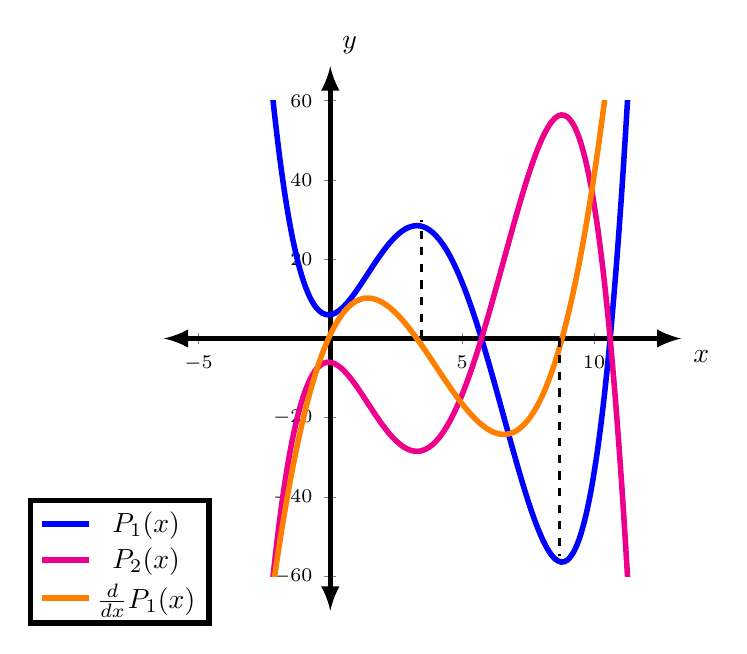
\begin{tikzpicture}
  \begin{axis}[
      samples=70,
      smooth,
      line width=2pt,
      domain=-4:12,
      legend pos=south west,
      legend style={
        anchor=east
      },
      width=0.6\textwidth,
      height=3in,
      axis lines=middle,
      xmin=-5,
      xmax=12,
      ymin=-60,
      ymax=60,
        scaled ticks=false,
        ticklabel style={font=\scriptsize},
        xlabel=$x$,
        ylabel=$y$,
        axis line style={
          latex-latex,
          shorten >=-12.5pt,
          shorten <=-12.5pt,
        },
        xlabel style={at={(ticklabel* cs:1)}, xshift=12.5pt, anchor=north west},
        ylabel style={at={(ticklabel* cs:1)}, yshift=12.5pt, anchor=south west},
    ]
    
    \addplot[color=blue] {0.125 * x^4 -2* x^3 + 7 * x^2 + x + 6};  
    \addlegendentry{\(P_1(x)\)}
    \addplot[color=magenta] {-0.125 * x^4 +2* x^3 - 7 * x^2 - x - 6};
    \addlegendentry{\(P_2(x)\)}
    \addplot[color=orange] {0.5 * x^3 -6* x^2 + 14 * x + 1};
    \addlegendentry{\(\frac{d}{dx}P_1(x)\)}
    \draw[dashed,line width=1pt] (3.45,0) -- (3.45,30);
    \draw[dashed,line width=1pt] (8.7,0) -- (8.7,-55);
  \end{axis}
\end{tikzpicture}
%
\caption{Quartics}
\label{fig.quartic}
\end{figure}
